%% forked from the following reference document provided by IEEE>
%%
%% bare_jrnl.tex
%% V1.4b
%% 2015/08/26
%% by Michael Shell
%% see http://www.michaelshell.org/
%% for current contact information.
%% Support sites:
%% http://www.michaelshell.org/tex/ieeetran/
%% http://www.ctan.org/pkg/ieeetran
%% and
%% http://www.ieee.org/

\documentclass[journal]{IEEEtran}

% If IEEEtran.cls has not been installed into the LaTeX system files,
% manually specify the path to it like:
% \documentclass[journal]{../sty/IEEEtran}
%\usepackage[showframe]{geometry}
%LPR: This chunk corrects a nasty bug in the IEEEtran biblography section.
\makeatletter
\def\endthebibliography{%
	\def\@noitemerr{\@latex@warning{Empty `thebibliography' environment}}%
	\endlist
}
\makeatother

%LPR: Insert the core extra packages.
%LPR: Uncomment parts of that file based upon your needs.
% Some very useful LaTeX packages include:
% (uncomment the ones you want to load)

% *** MISC UTILITY PACKAGES ***
%\usepackage{ifpdf}
% Heiko Oberdiek's ifpdf.sty is very useful if you need conditional
% compilation based on whether the output is pdf or dvi.
% usage:
% \ifpdf
%   % pdf code
% \else
%   % dvi code
% \fi
% The latest version of ifpdf.sty can be obtained from:
% http://www.ctan.org/pkg/ifpdf
% Also, note that IEEEtran.cls V1.7 and later provides a builtin
% \ifCLASSINFOpdf conditional that works the same way.
% When switching from latex to pdflatex and vice-versa, the compiler may
% have to be run twice to clear warning/error messages.


% *** CITATION PACKAGES ***
%\usepackage{cite}
\usepackage[noadjust]{cite}
% cite.sty was written by Donald Arseneau
% V1.6 and later of IEEEtran pre-defines the format of the cite.sty package
% \cite{} output to follow that of the IEEE. Loading the cite package will
% result in citation numbers being automatically sorted and properly
% "compressed/ranged". e.g., [1], [9], [2], [7], [5], [6] without using
% cite.sty will become [1], [2], [5]--[7], [9] using cite.sty. cite.sty's
% \cite will automatically add leading space, if needed. Use cite.sty's
% noadjust option (cite.sty V3.8 and later) if you want to turn this off
% such as if a citation ever needs to be enclosed in parenthesis.
% cite.sty is already installed on most LaTeX systems. Be sure and use
% version 5.0 (2009-03-20) and later if using hyperref.sty.
% The latest version can be obtained at:
% http://www.ctan.org/pkg/cite
% The documentation is contained in the cite.sty file itself.


% *** GRAPHICS RELATED PACKAGES ***
\ifCLASSINFOpdf
  \usepackage[pdftex]{graphicx}
  % declare the path(s) where your graphic files are
  \graphicspath{{pdf/}{jpg/}{png/}}
  % and their extensions so you won't have to specify these with
  % every instance of \includegraphics
  % \DeclareGraphicsExtensions{.pdf,.jpg,.png}
\else
  % or other class option (dvipsone, dvipdf, if not using dvips). graphicx
  % will default to the driver specified in the system graphics.cfg if no
  % driver is specified.
  % \usepackage[dvips]{graphicx}
  % declare the path(s) where your graphic files are
  % \graphicspath{{../eps/}}
  % and their extensions so you won't have to specify these with
  % every instance of \includegraphics
  % \DeclareGraphicsExtensions{.eps}
\fi
% graphicx was written by David Carlisle and Sebastian Rahtz. It is
% required if you want graphics, photos, etc. graphicx.sty is already
% installed on most LaTeX systems. The latest version and documentation
% can be obtained at: 
% http://www.ctan.org/pkg/graphicx
% Another good source of documentation is "Using Imported Graphics in
% LaTeX2e" by Keith Reckdahl which can be found at:
% http://www.ctan.org/pkg/epslatex
%
% latex, and pdflatex in dvi mode, support graphics in encapsulated
% postscript (.eps) format. pdflatex in pdf mode supports graphics
% in .pdf, .jpeg, .png and .mps (metapost) formats. Users should ensure
% that all non-photo figures use a vector format (.eps, .pdf, .mps) and
% not a bitmapped formats (.jpeg, .png). The IEEE frowns on bitmapped formats
% which can result in "jaggedy"/blurry rendering of lines and letters as
% well as large increases in file sizes.
%
% You can find documentation about the pdfTeX application at:
% http://www.tug.org/applications/pdftex


% *** MATH PACKAGES ***
\usepackage{amsmath}
% A popular package from the American Mathematical Society that provides
% many useful and powerful commands for dealing with mathematics.
%
% Note that the amsmath package sets \interdisplaylinepenalty to 10000
% thus preventing page breaks from occurring within multiline equations. Use:
%\interdisplaylinepenalty=2500
% after loading amsmath to restore such page breaks as IEEEtran.cls normally
% does. amsmath.sty is already installed on most LaTeX systems. The latest
% version and documentation can be obtained at:
% http://www.ctan.org/pkg/amsmath
\usepackage{cases}


% *** SPECIALIZED LIST PACKAGES ***
%\usepackage{algorithmic}
% algorithmic.sty was written by Peter Williams and Rogerio Brito.
% This package provides an algorithmic environment fo describing algorithms.
% You can use the algorithmic environment in-text or within a figure
% environment to provide for a floating algorithm. Do NOT use the algorithm
% floating environment provided by algorithm.sty (by the same authors) or
% algorithm2e.sty (by Christophe Fiorio) as the IEEE does not use dedicated
% algorithm float types and packages that provide these will not provide
% correct IEEE style captions. The latest version and documentation of
% algorithmic.sty can be obtained at:
% http://www.ctan.org/pkg/algorithms
% Also of interest may be the (relatively newer and more customizable)
% algorithmicx.sty package by Szasz Janos:
% http://www.ctan.org/pkg/algorithmicx



% *** ALIGNMENT PACKAGES ***
\usepackage{array}
% Frank Mittelbach's and David Carlisle's array.sty patches and improves
% the standard LaTeX2e array and tabular environments to provide better
% appearance and additional user controls. As the default LaTeX2e table
% generation code is lacking to the point of almost being broken with
% respect to the quality of the end results, all users are strongly
% advised to use an enhanced (at the very least that provided by array.sty)
% set of table tools. array.sty is already installed on most systems. The
% latest version and documentation can be obtained at:
% http://www.ctan.org/pkg/array

% IEEEtran contains the IEEEeqnarray family of commands that can be used to
% generate multiline equations as well as matrices, tables, etc., of high
% quality.


% *** SUBFIGURE PACKAGES ***
%\ifCLASSOPTIONcompsoc
%  \usepackage[caption=false,font=normalsize,labelfont=sf,textfont=sf]{subfig}
%\else
%  \usepackage[caption=false,font=footnotesize]{subfig}
%\fi
% subfig.sty, written by Steven Douglas Cochran, is the modern replacement
% for subfigure.sty, the latter of which is no longer maintained and is
% incompatible with some LaTeX packages including fixltx2e. However,
% subfig.sty requires and automatically loads Axel Sommerfeldt's caption.sty
% which will override IEEEtran.cls' handling of captions and this will result
% in non-IEEE style figure/table captions. To prevent this problem, be sure
% and invoke subfig.sty's "caption=false" package option (available since
% subfig.sty version 1.3, 2005/06/28) as this is will preserve IEEEtran.cls
% handling of captions.
% Note that the Computer Society format requires a larger sans serif font
% than the serif footnote size font used in traditional IEEE formatting
% and thus the need to invoke different subfig.sty package options depending
% on whether compsoc mode has been enabled.
%
% The latest version and documentation of subfig.sty can be obtained at:
% http://www.ctan.org/pkg/subfig


% *** FLOAT PACKAGES ***
%\usepackage{fixltx2e}
% fixltx2e, the successor to the earlier fix2col.sty, was written by
% Frank Mittelbach and David Carlisle. This package corrects a few problems
% in the LaTeX2e kernel, the most notable of which is that in current
% LaTeX2e releases, the ordering of single and double column floats is not
% guaranteed to be preserved. Thus, an unpatched LaTeX2e can allow a
% single column figure to be placed prior to an earlier double column
% figure.
% Be aware that LaTeX2e kernels dated 2015 and later have fixltx2e.sty's
% corrections already built into the system in which case a warning will
% be issued if an attempt is made to load fixltx2e.sty as it is no longer
% needed.
% The latest version and documentation can be found at:
% http://www.ctan.org/pkg/fixltx2e


\usepackage{stfloats}
% stfloats.sty was written by Sigitas Tolusis. This package gives LaTeX2e
% the ability to do double column floats at the bottom of the page as well
% as the top. (e.g., "\begin{figure*}[!b]" is not normally possible in
% LaTeX2e). It also provides a command:
\fnbelowfloat
% to enable the placement of footnotes below bottom floats (the standard
% LaTeX2e kernel puts them above bottom floats). This is an invasive package
% which rewrites many portions of the LaTeX2e float routines. It may not work
% with other packages that modify the LaTeX2e float routines. The latest
% version and documentation can be obtained at:
% http://www.ctan.org/pkg/stfloats
% Do not use the stfloats baselinefloat ability as the IEEE does not allow
% \baselineskip to stretch. Authors submitting work to the IEEE should note
% that the IEEE rarely uses double column equations and that authors should try
% to avoid such use. Do not be tempted to use the cuted.sty or midfloat.sty
% packages (also by Sigitas Tolusis) as the IEEE does not format its papers in
% such ways.
% Do not attempt to use stfloats with fixltx2e as they are incompatible.
% Instead, use Morten Hogholm'a dblfloatfix which combines the features
% of both fixltx2e and stfloats:
%
% \usepackage{dblfloatfix}
% The latest version can be found at:
% http://www.ctan.org/pkg/dblfloatfix




%\ifCLASSOPTIONcaptionsoff
%  \usepackage[nomarkers]{endfloat}
% \let\MYoriglatexcaption\caption
% \renewcommand{\caption}[2][\relax]{\MYoriglatexcaption[#2]{#2}}
%\fi
% endfloat.sty was written by James Darrell McCauley, Jeff Goldberg and 
% Axel Sommerfeldt. This package may be useful when used in conjunction with 
% IEEEtran.cls'  captionsoff option. Some IEEE journals/societies require that
% submissions have lists of figures/tables at the end of the paper and that
% figures/tables without any captions are placed on a page by themselves at
% the end of the document. If needed, the draftcls IEEEtran class option or
% \CLASSINPUTbaselinestretch interface can be used to increase the line
% spacing as well. Be sure and use the nomarkers option of endfloat to
% prevent endfloat from "marking" where the figures would have been placed
% in the text. The two hack lines of code above are a slight modification of
% that suggested by in the endfloat docs (section 8.4.1) to ensure that
% the full captions always appear in the list of figures/tables - even if
% the user used the short optional argument of \caption[]{}.
% IEEE papers do not typically make use of \caption[]'s optional argument,
% so this should not be an issue. A similar trick can be used to disable
% captions of packages such as subfig.sty that lack options to turn off
% the subcaptions:
% For subfig.sty:
% \let\MYorigsubfloat\subfloat
% \renewcommand{\subfloat}[2][\relax]{\MYorigsubfloat[]{#2}}
% However, the above trick will not work if both optional arguments of
% the \subfloat command are used. Furthermore, there needs to be a
% description of each subfigure *somewhere* and endfloat does not add
% subfigure captions to its list of figures. Thus, the best approach is to
% avoid the use of subfigure captions (many IEEE journals avoid them anyway)
% and instead reference/explain all the subfigures within the main caption.
% The latest version of endfloat.sty and its documentation can obtained at:
% http://www.ctan.org/pkg/endfloat
%
% The IEEEtran \ifCLASSOPTIONcaptionsoff conditional can also be used
% later in the document, say, to conditionally put the References on a 
% page by themselves.


% *** PDF, URL AND HYPERLINK PACKAGES ***
%\usepackage{url}
% url.sty was written by Donald Arseneau. It provides better support for
% handling and breaking URLs. url.sty is already installed on most LaTeX
% systems. The latest version and documentation can be obtained at:
% http://www.ctan.org/pkg/url
% Basically, \url{my_url_here}.


% *** Do not adjust lengths that control margins, column widths, etc. ***
% *** Do not use packages that alter fonts (such as pslatex).         ***
% There should be no need to do such things with IEEEtran.cls V1.6 and later.
% (Unless specifically asked to do so by the journal or conference you plan
% to submit to, of course. )

% correct bad hyphenation here
\hyphenation{op-tical net-works semi-conduc-tor}


%LPR: Extra packages YOU want to inclue go in this guy
%
% A few random packages that I think are particularly useful.
%

\usepackage{gensymb} % for \degree, etc.
\usepackage{xspace} % to fix \degree eating a space
% Redefine \degree to not eat a space based upon the \xspace package
\AtBeginDocument{%
	\let\OLDdegree\degree%
	\renewcommand{\degree}{\OLDdegree{}\xspace}%
}


\usepackage{xcolor} % for inkscape figures

% This handles warnings related to using the \input command on PDFs generated
% by inkscape's SVG->TEX conversion tool.
\pdfsuppresswarningpagegroup=1

% My mangled attempt at figuring out how to make footnotes place nicely with
% tables.
\usepackage{footnote}
\makesavenoteenv{tabular}
\makesavenoteenv{table}

% For the helper macros used to control markup while editing.
%
% This document is used to setup the flags we use to remove/show bits of the
% paper when writing working drafts.
%

\newif\ifLPRfmtDRAFT
\newif\ifLPRfmtHIGHLIGHTS
\newif\ifLPRfmtNOAUTH

% use to do disable/enable sections of text
\newif\ifNO
\newif\ifYES
\YEStrue

%%%%%
% Control Flags
%%%%%
% Comment these lines to change the behavior of the markup generation.
%
% Description:
%   fmtHIGHLITS controls the appearance of \editB, \editR, etc.
%       true => colored text, false => default black text
%   fmtNOAUTH disables and enables authors in both the title and afterward
%       true => authors hidden, false => authors visible
%   fmtDRAFT
%       true => \todo items visible in expanded page margins
%       false => \todo notes stripped, document width unchanged
%%%%%
\LPRfmtHIGHLIGHTStrue
%\LPRfmtNOAUTHtrue
\LPRfmtDRAFTtrue


\ifLPRfmtDRAFT
	%\usepackage{showframe} % used if you want to show outlines on the page margins

	\usepackage[colorinlistoftodos]{todonotes}
	% For color box on final page of self notes.
	\usepackage{mdframed}
	\usepackage{scrtime}
	\usepackage{soul}

	% Formating decisions for the TODO notes stuff that ends up at the end of the paper.
	\mdfdefinestyle{notesstyle}{%
		linecolor=red,frametitlerule=true,
		backgroundcolor=red!15}
	\mdfdefinestyle{outlinestyle}{%
		linecolor=green,frametitlerule=true,
		backgroundcolor=green!15}
	
	%\presetkeys{todonotes}{color=green!30, linecolor=red!90, size=\small, figwidth=3.4in}{}
	%\setlength{\marginparwidth}{1.4cm}

	\presetkeys{todonotes}{color=blue!15, linecolor=red!90, size=\footnotesize, figwidth=3.4in}{}
	\setlength{\marginparwidth}{0.8in}	% new margin size
	\setlength{\marginparpush}{0in}		% spacing between margin notes
	\addtolength{\paperwidth}{\marginparwidth}	% make the page bigger for the margins
	\addtolength{\hoffset}{0.5\marginparwidth}	% and make the page symetric for the margin
	
	\makeatletter
	\if@todonotes@disabled
		\newcommand{\hlfix}[2]{#1}
	\else
		\newcommand{\hlfix}[2]{\texthl{#1}\todo{#2}{}}
	\fi
	\makeatother
\else
	\makeatletter
	\newcommand{\hlfix}[2]{{}}
	\newcommand{\todo}[1]{{}}
	\makeatother
\fi


\ifLPRfmtHIGHLIGHTS
	\colorlet{editColorBlue}{blue!100!}
	\colorlet{editColorRed}{red!100!}
	\definecolor{editColorGreen}{RGB}{0,127,0}
	\definecolor{editColorRedRed}{RGB}{192,0,128}
	\definecolor{editColorBlueBlue}{RGB}{0,96,192}
	
	\newcommand{\editB}[1]{{\color{editColorBlue}#1}}
	\newcommand{\editR}[1]{{\color{editColorRed}#1}}
	\newcommand{\editG}[1]{{\color{editColorGreen}#1}}
	\newcommand{\editBB}[1]{{\color{editColorBlueBlue}#1}}
	\newcommand{\editRR}[1]{{\color{editColorRedRed}#1}}

	\newcommand{\dummy}[1][cite]{\cite{FooBar}\todo{#1}\xspace}
\else
	\newcommand{\editB}[1]{#1}
	\newcommand{\editR}[1]{#1}
	\newcommand{\editG}[1]{#1}
	\newcommand{\editBB}[1]{#1}
	\newcommand{\editRR}[1]{#1}
	\newcommand{\dummy}[1][cite]{\cite{FooBar}\todo{#1}\xspace}
	%\newcommand{\dummy}[1][CITE]{\texthl{!!}\cite{FooBar}\texthl{!!}\todo{#1}\xspace}
\fi




\begin{document}
% paper title
% Titles are generally capitalized except for words such as a, an, and, as,
% at, but, by, for, in, nor, of, on, or, the, to and up, which are usually
% not capitalized unless they are the first or last word of the title.
% Linebreaks \\ can be used within to get better formatting as desired.
% Do not put math or special symbols in the title.
\title{A Pretty Great Thing: \\Or, Why You Should Hire Me}

% author names and IEEE memberships
% note positions of commas and nonbreaking spaces ( ~ ) LaTeX will not break
% a structure at a ~ so this keeps an author's name from being broken across
% two lines.
% use \thanks{} to gain access to the first footnote area
% a separate \thanks must be used for each paragraph as LaTeX2e's \thanks
% was not built to handle multiple paragraphs
%\author{Michael~Shell,~\IEEEmembership{Member,~IEEE,}
%        John~Doe,~\IEEEmembership{Fellow,~OSA,}
%        and~Jane~Doe,~\IEEEmembership{Life~Fellow,~IEEE}% <-this % stops a space
\ifLPRfmtNOAUTH
\author{}% None of that if we're hiding authorship information.
\else
\author{Luke~Renaud,~\IEEEmembership{Student~Member,~IEEE,}
		Your~Labmate,~%\IEEEmembership{Student~Member,~IEEE,}
%		Your~Other~Labmate,~%\IEEEmembership{Student~Member,~IEEE,}
		Your~Professor,~\IEEEmembership{Senior~Member,~IEEE,}% <-this % stops a space
%\thanks{M. Shell was with the Department
%of Electrical and Computer Engineering, Georgia Institute of Technology, Atlanta,
%GA, 30332 USA e-mail: (see http://www.michaelshell.org/contact.html).}% <-this % stops a space
%\thanks{L. Renaud, Y. Labmate, and Y. Professor are with the School of Electrical Engineering and Computer Science, My University, City, ST, ZIPCODE USA (e-mail: l_renaud@univ.edu; y_labmate@univ.edu; y_professor@univ.edu).}% <-this % stops a space
%\thanks{Manuscript received April 19, 2005; revised August 26, 2015.}%
}
\fi

% note the % following the last \IEEEmembership and also \thanks - 
% these prevent an unwanted space from occurring between the last author name
% and the end of the author line. i.e., if you had this:
% 
% \author{....lastname \thanks{...} \thanks{...} }
%                     ^------------^------------^----Do not want these spaces!
%
% a space would be appended to the last name and could cause every name on that
% line to be shifted left slightly. This is one of those "LaTeX things". For
% instance, "\textbf{A} \textbf{B}" will typeset as "A B" not "AB". To get
% "AB" then you have to do: "\textbf{A}\textbf{B}"
% \thanks is no different in this regard, so shield the last } of each \thanks
% that ends a line with a % and do not let a space in before the next \thanks.
% Spaces after \IEEEmembership other than the last one are OK (and needed) as
% you are supposed to have spaces between the names. For what it is worth,
% this is a minor point as most people would not even notice if the said evil
% space somehow managed to creep in.


% The paper headers
%\markboth{IEEE Transactions on Circuits and Systems---II: Express Briefs,~Vol.~\#\#, No.~\#, Month~\#\#\#\#}%
\markboth{IEEE Transactions on Templates---I: Regular Papers,~Vol.~\#\#, No.~\#, Month~\#\#\#\#}{Renaud \MakeLowercase{\textit{et al.}}: \<~PAPER TITLE GOES HERE\>}
% The only time the second header will appear is for the odd numbered pages
% after the title page when using the twoside option.
% 
% *** Note that you probably will NOT want to include the author's ***
% *** name in the headers of peer review papers.                   ***
% You can use \ifCLASSOPTIONpeerreview for conditional compilation here if
% you desire.

% If you want to put a publisher's ID mark on the page you can do it like
% this:
%\IEEEpubid{0000--0000/00\$00.00~\copyright~2015 IEEE}
% Remember, if you use this you must call \IEEEpubidadjcol in the second
% column for its text to clear the IEEEpubid mark.

% make the title area
\maketitle

% As a general rule, do not put math, special symbols or citations
% in the abstract or keywords.
\begin{abstract}
Cras ut justo quis dui dignissim feugiat. Quisque dapibus, nisl id maximus hendrerit, enim neque ullamcorper nisl, in vulputate orci magna at ex. Aliquam lacinia neque augue, sit amet elementum ex ullamcorper vitae. Sed finibus, erat a porta lacinia, augue velit pretium justo, sit amet blandit enim arcu vel erat. Quisque turpis nisl, dictum non tellus iaculis, gravida aliquet lorem. \hlfix{Curabitur eget rutrum nunc.}{noted} In hac habitasse platea dictumst. Nulla consequat augue ac elit vulputate scelerisque. Etiam rutrum, mauris semper tempor consectetur, quam est hendrerit leo, ut tristique sem lacus quis magna. Praesent vestibulum orci libero, vel dignissim urna tristique ut. Etiam interdum fringilla justo ultrices molestie. Quisque rutrum vestibulum blandit. Vivamus rutrum convallis nisi ut porta. Pellentesque ex dolor, condimentum ullamcorper fringilla sit amet, fermentum quis velit. Nam nec orci bibendum, aliquam turpis ut, feugiat nisl. Maecenas finibus orci non purus fermentum tincidunt.%
\ifLPRfmtDRAFT\footnote{Compiled on \today\: at \thistime}\fi
\end{abstract}%


% Note that keywords are not normally used for peerreview papers.
\editB{%
\begin{IEEEkeywords}
TBD
\end{IEEEkeywords}%
}

% For peer review papers, you can put extra information on the cover
% page as needed:
% \ifCLASSOPTIONpeerreview
% \begin{center} \bfseries EDICS Category: 3-BBND \end{center}
% \fi
%
% For peerreview papers, this IEEEtran command inserts a page break and
% creates the second title. It will be ignored for other modes.
\IEEEpeerreviewmaketitle

\section{Introduction}\label{sec:10-intro}%
\IEEEPARstart{L}{orem} ipsum dolor sit amet, consectetur adipiscing elit. Integer ut mi sem. Vestibulum laoreet, velit non posuere rhoncus, massa enim tempus arcu, in sodales massa lorem ut arcu. Cras metus arcu, sagittis non orci eget, scelerisque volutpat ipsum. In ac dolor quis risus auctor aliquet ac non ex. Sed nec urna cursus, fringilla orci sit amet, dignissim mauris. Donec interdum lobortis ipsum, vel auctor diam volutpat hendrerit. Duis ex quam, faucibus id pharetra at, convallis ut tortor. Morbi ultrices posuere ligula, tincidunt scelerisque ligula semper ornare. Donec nec lorem porttitor, gravida orci eu, ultricies metus \dummy. Donec vestibulum, orci nec placerat porttitor, nisl mi hendrerit justo, a mattis neque mauris in nisl. Nunc lobortis, dui hendrerit accumsan cursus, lorem velit auctor ligula, pharetra faucibus tortor tellus suscipit arcu. Nam eget pulvinar nisl. Donec ornare blandit purus vel viverra. Nullam egestas convallis neque et laoreet. Proin ac egestas ipsum.

\editG{%
\subsection{A green subsection}
Cras ut justo quis dui dignissim feugiat. Quisque dapibus, nisl id maximus hendrerit, enim neque ullamcorper nisl, in vulputate orci magna at ex. Aliquam lacinia neque augue, sit amet elementum ex ullamcorper vitae. Sed finibus, erat a porta lacinia, augue velit pretium justo, sit amet blandit enim arcu vel erat. Quisque turpis nisl, dictum non tellus iaculis, gravida aliquet lorem. Curabitur eget rutrum nunc. In hac habitasse platea dictumst. Nulla consequat augue ac elit vulputate scelerisque. Etiam rutrum, mauris semper tempor consectetur, quam est hendrerit leo, ut tristique sem lacus quis magna. Praesent vestibulum orci libero, vel dignissim urna tristique ut. Etiam interdum fringilla justo ultrices molestie. Quisque rutrum vestibulum blandit. Vivamus rutrum convallis nisi ut porta. Pellentesque ex dolor, condimentum ullamcorper fringilla sit amet, fermentum quis velit. Nam nec orci bibendum, aliquam turpis ut, feugiat nisl. Maecenas finibus orci non purus fermentum tincidunt.%
}

Nullam vel nibh at odio rutrum scelerisque in et ligula. Cras ut efficitur leo, et commodo sem. Fusce in felis vulputate, bibendum mauris in, varius felis\todo{eh?}. Praesent purus arcu, lobortis id enim at, rhoncus iaculis quam. Sed quis diam a felis sollicitudin consectetur ac eget dui. Phasellus laoreet, ex eget blandit faucibus, turpis risus aliquam ex, eu varius dolor eros nec justo. Vestibulum viverra nulla et lobortis cursus. Aliquam at elementum enim, ac scelerisque risus. Sed tristique, neque a iaculis volutpat, tortor urna pellentesque lorem, id lacinia magna felis ut neque. Duis pretium erat quis cursus consequat. Suspendisse non elit non dui varius mattis. Vivamus nec rutrum lectus. Fusce suscipit ultricies varius. Donec ac dui neque. Phasellus a eros ipsum.

Nullam laoreet tortor neque, sed scelerisque justo mollis at. Sed id rhoncus nulla. In sodales lobortis dolor in accumsan. Quisque vehicula sapien est, et aliquam lorem pretium eget. Donec id ante nec leo bibendum scelerisque. Nulla sed velit diam. In vulputate ac lacus ac vestibulum.

Pellentesque fermentum mauris diam, et porttitor tortor porta quis. Aliquam consequat, est et vulputate fermentum, mauris tortor maximus lorem, rhoncus volutpat tellus eros et nibh. In a pharetra dui. Vivamus quis justo metus. Morbi dictum lorem vitae elit tristique pellentesque. Proin elementum placerat tortor vitae auctor. Ut cursus urna nec congue lobortis. Nulla facilisi. Cras maximus lacinia felis et maximus. Nam faucibus convallis sodales. 

\section{Theory of Operation}\label{sec:20-theory}
Lorem ipsum dolor sit amet, consectetur adipiscing elit. In non pulvinar dolor. Fusce id ipsum et neque blandit pharetra eget vitae quam. Pellentesque habitant morbi tristique senectus et netus et malesuada fames ac turpis egestas. Nullam egestas fermentum justo at rhoncus. Nunc eget suscipit quam. Duis non arcu at sem consequat egestas sed id est. Phasellus eget maximus massa. Suspendisse consectetur semper faucibus. Praesent a eros vel elit rutrum accumsan. Vestibulum laoreet pretium nulla a tempus. Nunc accumsan lacus non pulvinar vulputate. Aliquam sodales in enim vel porta.

\begin{figure}[t]
	\centering
	%\input{drawings/pdf_frominkscape.pdf_tex}
	%\includegraphics[width=3.4in,trim={0pt 0pt 0pt 0pt},clip]{figures/normal_pdf_or_file}
	\missingfigure{A figure I don't have}
	\caption{I really should put something here.}
	\label{fig:theory_csamp_schematic}
\end{figure}%
%
\subsection{Preventing Nuclear War}
Hello?... Uh... Hello D-- uh hello Dmitri? Listen uh uh I can't hear too well. Do you suppose you could turn the music down just a little?... Oh-ho, that's much better... yeah... huh... yes... Fine, I can hear you now, Dmitri... Clear and plain and coming through fine... I'm coming through fine, too, eh?... Good, then... well, then, as you say, we're both coming through fine... Good... Well, it's good that you're fine and... and I'm fine... I agree with you, it's great to be fine... a-ha-ha-ha-ha... Now then, Dmitri, you know how we've always talked about the possibility of something going wrong with the Bomb... The \textit{Bomb}, Dmitri... The \textit{hydrogen} bomb!... Well now, what happened is... ahm... one of our base commanders, he had a sort of... well, he went a little funny in the head... you know... just a little... funny. And, ah... he went and did a silly thing... Well, I'll tell you what he did. He ordered his planes... to attack your country... Ah... Well, let me finish, Dmitri... Let me finish, Dmitri... Well listen, how do you think I feel about it?... Can you \textit{imagine} how I feel about it, Dmitri?... Why do you think I'm calling you? Just to say hello?... \textit{Of course} I like to speak to you!... \textit{Of course} I like to say hello!... Not now, but anytime, Dmitri. I'm just calling up to tell you something terrible has happened... It's a \textit{friendly} call. Of course it's a friendly call... Listen, if it wasn't friendly... you probably wouldn't have even got it... They will \textit{not} reach their targets for at least another hour... I am... I am positive, Dmitri... Listen, I've been all over this with your ambassador. It is not a trick... Well, I'll tell you. We'd like to give your air staff a complete run-down on the targets, the flight plans, and the defensive systems of the planes... Yes! I mean i-i-i-if we're unable to recall the planes, then... I'd say that, ah... well, ah... we're just gonna have to help you destroy them, Dmitri... I know they're our boys... All right, well listen now. Who should we call?... \textit{Who} should we call, Dmitri? The... wha-whe, the People... you, sorry, you faded away there... The People's Central Air Defense Headquarters... Where is that, Dmitri?... In Omsk... Right... Yes... Oh, you'll call them first, will you?... Uh-huh... Listen, do you happen to have the phone number on you, Dmitri?... Whe-ah, what? I see, just ask for Omsk information... Ah-ah-eh-uhm-hm... I'm sorry, too, Dmitri... I'm very sorry... \textit{All right}, you're sorrier than I am, but I am as sorry as well... I am as sorry as you are, Dmitri! Don't say that you're more sorry than I am, because I'm capable of being just as sorry as you are... So we're both sorry, all right?... All right. 

\editR{%
\subsection{Subsection in Red}%
Suspendisse nunc diam, venenatis at nisl quis, elementum eleifend diam. Nam sed molestie odio. Quisque maximus est vel arcu ultrices posuere. In hac habitasse platea dictumst. Nunc in sapien vel arcu mollis laoreet quis at sapien. Praesent nunc urna, tincidunt tempus leo ac, fringilla imperdiet nibh. Duis venenatis imperdiet laoreet. Sed at erat erat. Maecenas vitae euismod magna.%
%
\begin{IEEEeqnarray}{rl}
	\angle H_{x}(\delta, \gamma, {}&G_x) = \frac{\pi}{2}-\arctan 
	\Bigg[ \frac{1}{Q}
		\frac{
			(1+\delta)
		}{
			1 - ( 1 + \delta )^2  (1 + \gamma)
		}
	\Bigg]
	\label{eqn:theory_csamp_phase}\\
	\left| H_{x}(\delta, \gamma,\right.&\left.G_x) \right| = 
	\frac{g_{m,x}}{G_x} \times \IEEEnonumber \\
	{}&\frac{
		\left| 1 + \delta \right|
	}{\sqrt{
		(1 + \delta)^2 + Q^2 \big[ 1 - ( 1 + \delta )^2  (1 + \gamma)\big]^2
	}}
	\label{eqn:theory_csamp_mag}
\end{IEEEeqnarray}%
%
Aliquam ullamcorper accumsan diam, ac egestas ante porta et. Mauris lacinia, dui id suscipit pharetra, tellus purus hendrerit tellus, vel bibendum felis diam ut massa. Nullam id ex in mi iaculis sodales et ut ipsum. Nulla mollis purus in risus consectetur, at rutrum nunc ullamcorper. Integer id consectetur ex, sed elementum ligula. Aenean maximus feugiat turpis non finibus. Ut lacinia finibus diam ac pellentesque. Sed ipsum ligula, hendrerit a convallis sit amet, pellentesque at purus. Vestibulum condimentum bibendum tempus. Aenean in pulvinar ipsum. Etiam tempus finibus quam, dapibus tempor nunc elementum blandit. Proin consectetur finibus ligula, sed malesuada quam pulvinar ultrices. Donec ultricies, metus eu ullamcorper dictum, augue risus viverra urna, in posuere nisi dui vel risus. Phasellus ac viverra nisl. Aenean faucibus ligula nisl, venenatis lacinia ex pretium egestas. Praesent nunc tellus, ultrices nec augue quis, maximus aliquam sem.%

Sed malesuada turpis vitae pharetra tempor\todo{This is clearly not english.}. \editRR{Etiam iaculis quis enim sodales tincidunt. Duis eu tellus lorem. Aenean viverra purus eu erat cursus, non imperdiet sapien lacinia.} In gravida nulla vitae mattis semper. Sed libero ipsum, viverra vel gravida eu, varius at lectus. Nullam placerat commodo massa at congue. Donec volutpat erat vel enim condimentum posuere id sed mauris. Fusce aliquam, magna at venenatis vehicula, augue nulla molestie dolor, eget lacinia turpis diam ut odio.

Morbi quis est sed mi dictum blandit ornare non diam. Vestibulum congue, metus in posuere pulvinar, turpis quam imperdiet mauris, vel faucibus lectus nulla quis ipsum. Nam sagittis urna aliquam, lobortis libero quis, viverra lorem. Ut eget laoreet odio. Maecenas eget ligula lorem. Orci varius natoque penatibus et magnis dis parturient montes, nascetur ridiculus mus. Aenean eros nibh, varius sed justo in, hendrerit vulputate nulla.%
}

\editB{%
\section{Example Section}
One, our hopes for recalling the 843rd bomb wing are quickly being reduced to a very low order of probability.

Two, in less than fifteen minutes from now the Russkies will be making radar contact with the planes.

Three, when the do, they are going to go absolutely ape, and they're gonna strike back with everything they've got.

Four, if prior to this time, we have done nothing further to suppress their retaliatory capabilities, we will suffer virtual annihilation.

Now, five, if on the other hand, we were to immediately launch an all out and coordinated attack on all their airfields and missile bases we'd stand a damn good chance of catching them with their pants down. Hell, we got a five to one missile superiority as it is. We could easily assign three missiles to every target, and still have a very effective reserve force for any other contingency.

Now, six, an unofficial study which we undertook of this eventuality, indicated that we would destroy ninety percent of their nuclear capabilities. We would therefore prevail, and suffer only modest and acceptable civilian casualties from their remaining force which would be badly damaged and uncoordinated.
}

%\editG{%
\section{Conclusion}\label{sec:90-conclude}%
Mr. President, it is not only possible, it is essential. That is the whole idea of this machine, you know. Deterrence is the art of producing in the mind of the enemy... the \textbf{fear} to attack. And so, because of the automated and irrevocable decision-making process which rules out human meddling, the Doomsday machine is terrifying and simple to understand... and completely credible and convincing.

And! you really should go watch this movie.
%}

%\appendices
%\input{sections/110-apdx1.tex}
%\input{sections/120-apdx2.tex}

% An example of a floating figure using the graphicx package.
% Note that \label must occur AFTER (or within) \caption.
% For figures, \caption should occur after the \includegraphics.
% Note that IEEEtran v1.7 and later has special internal code that
% is designed to preserve the operation of \label w\marginparwidthithin \caption
% even when the captionsoff option is in effect. However, because
% of issues like this, it may be the safest practice to put all your
% \label just after \caption rather than within \caption{}.
%
% Reminder: the "draftcls" or "draftclsnofoot", not "draft", class
% option should be used if it is desired that the figures are to be
% displayed while in draft mode.
%
%\begin{figure}[!t]
%\centering
%\includegraphics[width=2.5in]{myfigure}
% where an .eps filename suffix will be assumed under latex, 
% and a .pdf suffix will be assumed for pdflatex; or what has been declared
% via \DeclareGraphicsExtensions.
%\caption{Simulation results for the network.}
%\label{fig_sim}
%\end{figure}

% Note that the IEEE typically puts floats only at the top, even when this
% results in a large percentage of a column being occupied by floats.

% An example of a double column floating figure using two subfigures.
% (The subfig.sty package must be loaded for this to work.)
% The subfigure \label commands are set within each subfloat command,
% and the \label for the overall figure must come after \caption.
% \hfil is used as a separator to get equal spacing.
% Watch out that the combined width of all the subfigures on a 
% line do not exceed the text width or a line break will occur.
%
%\begin{figure*}[!t]
%\centering
%\subfloat[Case I]{\includegraphics[width=2.5in]{box}%
%\label{fig_first_case}}
%\hfil
%\subfloat[Case II]{\includegraphics[width=2.5in]{box}%
%\label{fig_second_case}}
%\caption{Simulation results for the network.}
%\label{fig_sim}
%\end{figure*}
%
% Note that often IEEE papers with subfigures do not employ subfigure
% captions (using the optional argument to \subfloat[]), but instead will
% reference/describe all of them (a), (b), etc., within the main caption.
% Be aware that for subfig.sty to generate the (a), (b), etc., subfigure
% labels, the optional argument to \subfloat must be present. If a
% subcaption is not desired, just leave its contents blank,
% e.g., \subfloat[].

% An example of a floating table. Note that, for IEEE style tables, the
% \caption command should come BEFORE the table and, given that table
% captions serve much like titles, are usually capitalized except for words
% such as a, an, and, as, at, but, by, for, in, nor, of, on, or, the, to
% and up, which are usually not capitalized unless they are the first or
% last word of the caption. Table text will default to \footnotesize as
% the IEEE normally uses this smaller font for tables.
% The \label must come after \caption as always.
%
%\begin{table}[!t]
%% increase table row spacing, adjust to taste
%\renewcommand{\arraystretch}{1.3}
% if using array.sty, it might be a good idea to tweak the value of
% \extrarowheight as needed to properly center the text within the cells
%\caption{An Example of a Table}
%\label{table_example}
%\centering
%% Some packages, such as MDW tools, offer better commands for making tables
%% than the plain LaTeX2e tabular which is used here.
%\begin{tabular}{|c||c|}
%\hline
%One & Two\\
%\hline
%Three & Four\\
%\hline
%\end{tabular}
%\end{table}

% Note that the IEEE does not put floats in the very first column
% - or typically anywhere on the first page for that matter. Also,
% in-text middle ("here") positioning is typically not used, but it
% is allowed and encouraged for Computer Society conferences (but
% not Computer Society journals). Most IEEE journals/conferences use
% top floats exclusively. 
% Note that, LaTeX2e, unlike IEEE journals/conferences, places
% footnotes above bottom floats. This can be corrected via the
% \fnbelowfloat command of the stfloats package.

% use section* for acknowledgment
\if{false}
\section*{Acknowledgment}
The authors would like to thank...
\fi

% Can use something like this to put references on a page
% by themselves when using endfloat and the captionsoff option.
\ifCLASSOPTIONcaptionsoff
  \newpage
\fi

% trigger a \newpage just before the given reference
% number - used to balance the columns on the last page
% adjust value as needed - may need to be readjusted if
% the document is modified later
%\IEEEtriggeratref{8}
% The "triggered" command can be changed if desired:
%\IEEEtriggercmd{\enlargethispage{-5in}}

% references section
% The IEEEtran BibTeX style support page is at:
% http://www.michaelshell.org/tex/ieeetran/bibtex/
\bibliographystyle{IEEEtran}
% **** IEEE Bibliography STUFF ****
\bibliography{IEEEabrv,references}
%LPR: i.e. references.bib in this folder is your references database.
%LPR: I use JabRef to manage my references.

% Only show authors if fmtNOAUTH is false
\ifLPRfmtNOAUTH\else
	% biography section
% 
% If you have an EPS/PDF photo (graphicx package needed) extra braces are
% needed around the contents of the optional argument to biography to prevent
% the LaTeX parser from getting confused when it sees the complicated
% \includegraphics command within an optional argument. (You could create
% your own custom macro containing the \includegraphics command to make things
% simpler here.)
%\begin{IEEEbiography}[{\includegraphics[width=1in,height=1.25in,clip,keepaspectratio]{mshell}}]{Michael Shell}
% or if you just want to reserve a space for a photo:
%\newpage
\vspace{-0.5 cm}

\begin{IEEEbiography}[{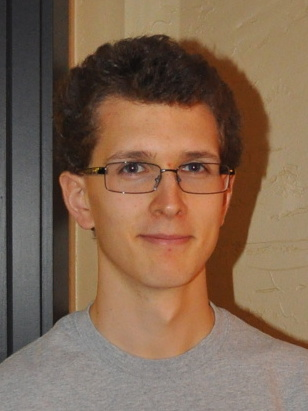
\includegraphics[width=1in,height=1.25in,clip,keepaspectratio]{photos/renaud.jpg}}]{Luke Renaud}
%\begin{IEEEbiographynophoto}{Luke Renaud}
(S’13) received the B.S. in Electrical Engineering \textit{summa cumme laude} with a from Washington State University in Pullman, WA in 2013. He is currently pursuing a Ph.D. in RF Microelectronics from Washington State University, Pullman, WA.

If you're reading this paragraph as a reviewer, then the person who submit the paper has forgotten to remove my template BIO from their document. You really should reject their paper, that's pretty sloppy.
%\end{IEEEbiographynophoto}
\vspace{-0.8 cm}
\end{IEEEbiography}

%\vfill

%\begin{IEEEbiography}[{\includegraphics[width=1in,height=1.25in,clip,keepaspectratio]{photos/ylabmate}}]{Your Labmate}
\begin{IEEEbiographynophoto}{Your Labmate}
Bio paragraph
\end{IEEEbiographynophoto}
%\end{IEEEbiography}
%\vspace{-0.8 cm}

%\begin{IEEEbiography}[{\includegraphics[width=1in,height=1.25in,clip,keepaspectratio]{photos/yprof}}]{Your Professor}
\begin{IEEEbiographynophoto}{Your Professor}
Bio paragraph
\end{IEEEbiographynophoto}
%\end{IEEEbiography}

% insert where needed to balance the two columns on the last page with
% biographies
%\newpage

%\begin{IEEEbiographynophoto}{Jane Doe}
%Biography text here.
%\end{IEEEbiographynophoto}

% You can push biographies down or up by placing
% a \vfill before or after them. The appropriate
% use of \vfill depends on what kind of text is
% on the last page and whether or not the columns
% are being equalized.

\vfill

% Can be used to pull up biographies so that the bottom of the last one
% is flush with the other column.
%\enlargethispage{-5in}

\fi

% Add the random todo items to the end of the document if we want them.
\ifLPRfmtDRAFT
	
\vfill
\pagebreak

\hrule

\begin{mdframed}[style=outlinestyle,frametitle={Inital Outline:}]
\begin{itemize}
	\item introduction/background
	\begin{itemize}
		\item existing topologies
		\item challenges and characteristics \textbf{[elaborate]}
	\end{itemize}
	\item block diagram overview
	\item design discussions (theory)
	\item Control Overview
	\item Measurement results
	\item Conclusion
\end{itemize}
\end{mdframed}

\begin{mdframed}[style=notesstyle,frametitle={Remaining TODO items:}]
\begin{itemize}
		\item update biographies
	\item align final biographies properly (last step before submitting.)
	\item a random note to myself
\end{itemize}
\end{mdframed}

\listoftodos


\fi

% that's all folks
\end{document}

